\iffalse
\author{EE24BTECH11047}
\section{xe}
\chapter{2021}
\fi
    \item Match the heat treatment processes given in Column I with the most suitable outcomes in Column II. \\
    \begin{tabular}{c c}
        
        Column I & Column II \\
        
        (P) Quenching & (1) Hardens the steel \\
        (Q) Annealing & (2) Softens the cold worked steel \\
        (R) Tempering & (3) Softens the steel \\
        (S) Carburizing & (4) Increases the surface hardness of steel \\
        
    \end{tabular}
    
    \begin{enumerate}
        \item P-3; Q-2; R-1; S-4
        \item P-2; Q-3; R-4; S-1
        \item P-3; Q-1; R-4; S-2 
        \item P-1; Q-3; R-4; S-2
    \end{enumerate}

    \item A co-joined cross-ply laminate composite, as shown in the figure, is distorted upon heating. What are the resultant shapes of layers XY and YZ? \\
    \begin{figure}[!ht]
\centering
\resizebox{1\textwidth}{!}{%
\begin{circuitikz}
\tikzstyle{every node}=[font=\normalsize]
\draw [short] (2,7.5) -- (4.75,9);
\draw [short] (3.5,5.5) -- (6.25,7);
\draw [short] (2,7.5) -- (3.5,5.5);
\draw [short] (4.75,9) -- (6.25,7);
\draw [short] (6.25,7) -- (6.25,6);
\draw [short] (3.5,5.5) -- (3.5,4.5);
\draw [short] (3.5,4.5) -- (6.25,6);
\draw [short] (2,6.5) -- (3.5,4.5);
\draw [short] (2,7.5) -- (2,6.5);
\draw [short] (2,7) -- (3.5,5);
\draw [short] (3.5,5) -- (6.25,6.5);
\draw [short] (2.75,7.5) -- (3.75,6);
\node [font=\LARGE] at (3.75,6.25) {};
\draw [short] (3.25,7.75) -- (4.25,6.25);
\draw [short] (3.75,8) -- (4.75,6.5);
\draw [short] (4.25,8.25) -- (5.25,6.75);
\draw [short] (4.75,8.5) -- (5.75,7);
\node [font=\normalsize] at (3.5,4.25) {\textbf{Y}};
\node [font=\normalsize] at (6.5,5.75) {\textbf{Z}};
\node [font=\normalsize] at (1.75,6.25) {\textbf{X}};
\draw  (3.75,5.5) circle (0cm);
\node [font=\Huge] at (3.75,5.5) {\textbf{.}};
\node [font=\Huge] at (4.25,5.75) {\textbf{.}};
\node [font=\Huge] at (4.75,6) {\textbf{.}};
\node [font=\Huge] at (4.5,6) {\textbf{.}};
\node [font=\Huge] at (4,5.75) {\textbf{.}};
\node [font=\Huge] at (5,6.25) {\textbf{.}};
\node [font=\Huge] at (5.25,6.25) {\textbf{.}};
\node [font=\Huge] at (5.5,6.5) {\textbf{.}};
\node [font=\Huge] at (5.75,6.5) {\textbf{.}};
\node [font=\Huge] at (6,6.75) {\textbf{.}};
\node [font=\Huge] at (2.5,6.25) {\textbf{.}};
\node [font=\Huge] at (2.75,6) {\textbf{.}};
\node [font=\Huge] at (3,5.5) {\textbf{.}};
\node [font=\Huge] at (2.25,6.5) {\textbf{.}};
\node [font=\Huge] at (3.25,5.25) {\textbf{.}};
\node [font=\Huge] at (2.25,6.5) {\textbf{.}};
\draw [->, >=Stealth] (2.5,5) -- (3.75,5.5);
\draw [->, >=Stealth] (2.5,5) -- (2.5,6);
\draw [->, >=Stealth] (5.25,4.5) -- (4,5.5);
\draw [->, >=Stealth] (5.25,4.5) -- (5.25,5.75);
\node [font=\normalsize, rotate around={-45:(0,0)}] at (2.25,5) {Ceramic fiber};
\node [font=\normalsize] at (5.5,4.25) {polymer matrix};
\end{circuitikz}
}%

\label{fig:my_label}
\end{figure}
    
    \begin{enumerate}
        \item X \raisebox{1ex}{\rule{0.5cm}{0.4pt}} Y, Y \begin{tikzpicture}
    \draw (0,0) arc[start angle=220, end angle=320, radius=0.5cm];
\end{tikzpicture} Z
        \item X \begin{tikzpicture}
    \draw (0,0) arc[start angle=220, end angle=320, radius=0.5cm];
\end{tikzpicture} Y, Y \raisebox{1ex}{\rule{0.5cm}{0.4pt}} Z
        \item X \begin{tikzpicture}
    \draw (0,0) arc[start angle=220, end angle=320, radius=0.5cm];
\end{tikzpicture} Y, Y \begin{tikzpicture}
    \draw (0,0) arc[start angle=40, end angle=140, radius=0.5cm];
\end{tikzpicture} Z
        \item X \begin{tikzpicture}
    \draw (0,0) arc[start angle=40, end angle=140, radius=0.5cm];
\end{tikzpicture} Y, Y \begin{tikzpicture}
    \draw (0,0) arc[start angle=220, end angle=320, radius=0.5cm];
\end{tikzpicture} Z
    \end{enumerate}

    \item X-ray diffraction peak broadening enables the estimation of
    \begin{enumerate}
        \item crystallite size of the material
        \item residual stresses in the material
        \item precise lattice parameter
        \item residual microstrains acting on the material
    \end{enumerate}
    \item Fe - 10 atom \% C austenite (fcc), having no Fe vacancies, has a lattice parameter of 4. Å. The density of austenite in g cm$^{-3}$ is \textbf{(round off to 2 decimal places)}. \\
    (Given: atomic weight of Fe = 55.85; atomic weight of C = 12.0; Avogadro's number = $6.023 \times 10^{23}$)

    \item An element transforms from $\alpha$ to $\beta$ at 773 K and 1 atm pressure with 912 J mol$^{-1}$ as enthalpy of transformation. The molar volumes of $\alpha$ and $\beta$ phases are 7 and 7.5 cm$^3$ mol$^{-1}$, respectively. Determine the difference in their internal energy at 773 K, independent of pressure. The amount of heat required for 10 g of transformation to occur at 723 K is \textbf{(round off to nearest integer)}. \\
    (Given: Atomic mass of $\alpha$ = 110.325 $\times 10^6$ Pa)

    \item A binary A-B alloy has $\alpha$ and $\beta$ phases at equilibrium. The ratio of weight fraction of A in $\alpha$ to $\beta$ is 4. The wt.\% of A in $\alpha$ and $\beta$ phases is 70 and 20, respectively. The wt.\% of B in the alloy is \textbf{(round off to nearest integer)}.

    \item During heating, Ti undergoes allotropic transformation from bcc to hcp at 882 $^{\circ}$C. The percent volume change accompanying this transformation is \textbf{(round off to 1 decimal place)}. \\
    (Given: atomic weight of Ti = 47.9; lattice parameter of bcc Ti = 0.332 nm; density of hcp Ti = 4.51 g cm$^{-3}$; Avogadro's number = $6.023 \times 10^{23}$)

    \item Vickers hardness test is performed with an indenter of square-base diamond pyramid having an included angle of 136$^{\circ}$ between the opposite faces of the pyramid. If the diagonal length is 0.5 mm and the average indentation depth is 0.015 mm, the Vickers hardness in kg mm$^{-2}$ is \textbf{(round off to nearest integer)}.

    \item The drift mobility of electron in an n-type Si crystal doped with $10^{16}$ cm$^{-3}$ phosphorus atoms is 1350 cm$^2$ V$^{-1}$ s$^{-1}$. The electrical conductivity in $\Omega$ m$^{-1}$ is \textbf{(round off to 2 decimal places)}. \\
    (Given: Intrinsic charge concentration of Si = $1.45 \times 10^{10}$ cm$^{-3}$; Charge of an electron, e = $1.6 \times 10^{-19}$ C)

    \item At 1000 K, the linear thermal expansion coefficients of graphite, parallel and perpendicular to the graphite layers, are 0.8 $\times 10^{-6}$ K$^{-1}$ and 29 $\times 10^{-6}$ K$^{-1}$, respectively. The percentage increase in the volume of graphite when the temperature rises from 100 K to 1100 K is \textbf{(round off to 2 decimal places)}.

    \item A certain ceramic material has a theoretical density and sintered density of 6.76 g cm$^{-3}$ and 6.69 g cm$^{-3}$, respectively. The green compact has 18 volume percent porosity. For a sintered cube of side 2 cm, the weight of the cubic green compact in cm is \textbf{(round off to 2 decimal places)}.

    \item When a metal (M) is immersed in de-aerated acid electrolyte, it polarizes anodically by 0.4 V. The M/M$^{2+}$ couple standard energy is 10$^{-4}$ A cm$^{-2}$ and A = 4 cm$^2$. Use a tafel slope of 0.12 V decade$^{-1}$ in the anodic reaction. Both anodic and cathodic reactions are under activation control. The rate of metal dissolution in A m$^{-2}$ is \textbf{(round off to 1 decimal place)}.

    \item A force $F = 40$ kN is applied on the hook as shown. The equivalent force-couple system at $B$ is
     \begin{figure}[!ht]
    \centering
    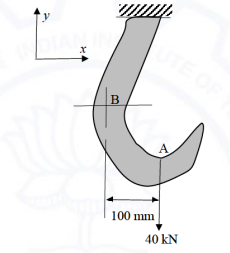
\includegraphics[width=4cm]{./GATE-yearwise/2021/figs/fig1.png}
    \end{figure}
    \begin{enumerate}
        \item 40 kN in $+y$ direction and $M = 0$
        \item 40 kN in $-y$ direction and $M = 0$
        \item 40 kN in $+y$ direction and $M = 4000$ Nm counter clockwise
        \item 40 kN in $+y$ direction and $M = 4000$ Nm clockwise
    \end{enumerate}
2
